\section{Preliminaries}
\label{sec:background}

\newcommand{\ivc}{\textit{IVC}}
\newcommand{\mivc}{\textit{MIVC}}
\newcommand{\bool}[0]{\mathit{bool}}
\newcommand{\reach}[0]{\mathit{R}}
\newcommand{\ite}[3]{\mathit{if}\ {#1}\ \mathit{then}\ {#2}\ \mathit{else}\ {#3}}

%\subsection{Transition Systems and Safety Properties}
Given a state space $U$, a transition system $(I,T)$ consists of an
initial state predicate $I : U \to \bool$ and a transition step
predicate $T : U \times U \to \bool$.
We define the notion of
reachability for $(I, T)$ as the smallest predicate $\reach : U \to
\bool$ which satisfies the following formulas:
\begin{gather*}
  \forall u.~ I(u) \Rightarrow \reach(u) \\
  \forall u, u'.~ \reach(u) \land T(u, u') \Rightarrow \reach(u')
\end{gather*}
A safety property $P : U \to \bool$ is a state predicate. A safety
property $P$ holds on a transition system $(I, T)$ if it holds on all
reachable states, i.e., $\forall u.~ \reach(u) \Rightarrow P(u)$,
written as $\reach \Rightarrow P$ for short. When this is the case, we
write $(I, T)\vdash P$. We assume the transition relation has the structure of a top-level conjunction.  Given $T(u, u') = T_1(u, u') \land \cdots \land T_n(u, u')$ we will write $T = \bigwedge_{i=1..n}T_i$ for short.
By further abuse of notation,
$T$ is identified with the set of its top-level conjuncts. Thus, $T_i \in
T$ means that $T_i$ is a top-level conjunct of $T$, and $S
\subseteq T$ means all top-level conjuncts of $S$ are top-level
conjuncts of $T$. When a top-level conjunct $T_i$ is removed from $T$, it is written as $T \setminus \{T_i\}$. Such a transition system can easily encode our example model in Section~\ref{sec:example}, where each equation defines a conjunct within $T$ that we will denote by the variable assigned; so, $T = \{$ {\small \texttt{a1\_below, a2\_below, a1\_above, a2\_above, one\_below, both\_above, doi\_on, on\_p}} $\}$.

The idea behind finding an IVC for a given property $P$ \cite{Ghass16} is based on inductive proof methods used in SMT-based model checking, such as $K$-induction and IC3/PDR \cite{NFM2012:KaGaTiWh, amla2005analysis, Een2011:PDR}. Generally, an IVC computation technique aims to determine, for any subset $S \subseteq T$, whether $P$ is provable by $S$. Then, a minimal subset that satisfies $P$ is seen as a minimal proof explanation called a minimal Inductive Validity Core.

\begin{definition}{\emph{Inductive Validity Core (\ivc)\cite{Ghass16}:}}
  \label{def:ivc}
  $S \subseteq T$ for $(I, T)\vdash P$ is an Inductive Validity Core,
  denoted by $\ivc(P, S)$, iff $(I, S) \vdash P $.
\end{definition}

\begin{definition}{\emph{Minimal Inductive Validity Core (\mivc) \cite{Ghass16}:}}
  \label{def:minimal-ivc}
  $S \subseteq T$ is a minimal Inductive Validity Core,
  denoted by $\mivc(P, S)$, iff ~$\ivc(P, S) \wedge \forall T_i \in S.~ (I, S\setminus\{ T_i \}) \nvdash P$.
\end{definition}


Note that, given $(I, T) \vdash P$, $P$ always has at least one \mivc, and it may also have many distinct \mivc s corresponding to different proof paths. To capture the latter, the \emph{all \mivc s ($AIVC$)} relation has been introduced in \cite{Murugesan16:renext}.
\begin{definition}{\emph{All \mivc s ($AIVC$):}}
    \label{def:allivcs}
    Given $(I, T) \vdash P$, $AIVC(P)$ is an association to all \mivc s for $P$:
    $$ AIVC(P) \equiv  \{\ S~|~S \subseteq T \land  MIVC(P, S)\} $$
\end{definition}

Figure~\ref{fig:ivcs} illustrates these notions by a graphical representation of IVCs for property $P = (\small{\texttt{on\_p}})$ in the example presented in Section~\ref{sec:example}. As shown in the picture, this property has two distinct \mivc s, which means the model satisfies $P$ in two different ways:  \texttt{\{\{a1\_below, one\_below, doi\_on, on\_p\}, \{a2\_below, one\_below, doi\_on, on\_p\}\}}, This is because in the implementation, the DOI is turned on when either of the altimeters is below the threshold, while our property states that they both must be below.
Note that there is a subset of model elements, $\{{\small \texttt{a1\_above, a2\_above, both\_above}}\}$, that does not show up in $AIVC(P)$. Elements in such a subset
do not affect the satisfaction of $P$.  In the complete ASW model in~\cite{HCW02:ase-deviation} there are additional properties that use these elements, but they are not necessary for the discussion in this paper.

%As you can see, distinct IVCs may have common elements.
%The intersection of all \mivc s is called the \emph{must} set for $P$.
%And, the other elements constitute a \emph{may} set for $P$ \cite{Murugesan16:renext}:
%\begin{itemize}
%  \item   $MUST (P) = \bigcap AIVC(P)$
%  \item  $MAY(P) = (\bigcup AIVC (P)) \setminus MUST(P)$
%  \item $IRR(P) = T \setminus (\bigcup AIVC(P))$
%\end{itemize}
%\noindent Given property $P$, functions $MUST$, $MAY$, and $IRR$ partition top-level conjuncts of $T$ (model elements) into three disjoint sets \emph{must}, \emph{may}, and \emph{irrelevant}, respectively. $IRR(P)$ returns portion of the model irrelevant to the satisfaction of $P$, which in our running example is $\varnothing$.
%We will make use of this intuition in Section~\ref{subsec:minimality}.

\begin{figure}[t]
 \centering
  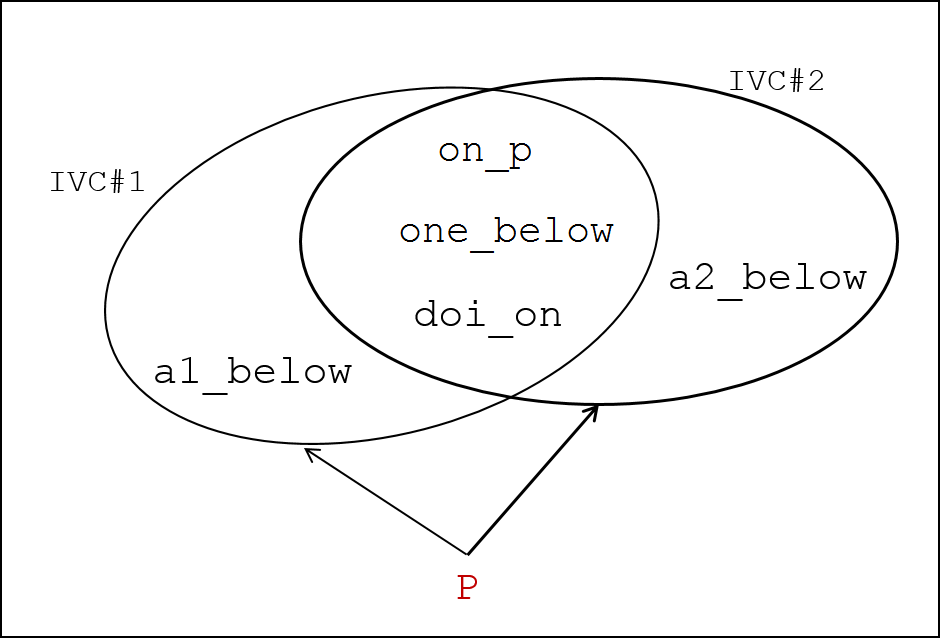
\includegraphics[width=0.9\columnwidth]{figs/ivcs.png}
  \label{fig:ivcs}
  \vspace{-0.1in}
  \caption{Graphical representation of \mivc s for the model in Figure\ref{fig:asw}
  with  $P = (\small{\texttt{on\_p}})$}
\end{figure}

%\subsection{Satisfiability}
%In this subsection, we provide a brief background on satisfiability problem.



